\documentclass[a4paper]{extarticle}
\usepackage[utf8]{inputenc}
\usepackage[a4paper, margin=1in]{geometry}

\usepackage{amssymb}
\usepackage{amsmath}
\usepackage{enumitem}
\usepackage{tcolorbox}
\usepackage{fancyhdr}
\usepackage{graphicx}
\usepackage{float}

\setlength{\parindent}{0em}
\setlength{\parskip}{0.4em}

\definecolor{theoremblue}{RGB}{1, 73, 124}
\definecolor{corollaryblue}{RGB}{70, 143, 175}
\definecolor{exampleblue}{RGB}{137, 194, 217}

\newtcolorbox{tbox}{colback=theoremblue!20,colframe=theoremblue,
boxrule=0pt,arc=0pt,boxsep=2pt,left=2pt,right=2pt,leftrule=2pt}

\newtcolorbox{cbox}{colback=corollaryblue!20,colframe=corollaryblue,
boxrule=0pt,arc=0pt,boxsep=2pt,left=2pt,right=2pt,leftrule=2pt}

\newtcolorbox{ebox}{colback=exampleblue!20,colframe=exampleblue,
boxrule=0pt,arc=0pt,boxsep=2pt,left=2pt,right=2pt,leftrule=2pt}

\title{EnpRisk - Lecture Notes Week 7}
\author{Ruben Schenk, ruben.schenk@inf.ethz.ch}
\date{\today}

\pagestyle{fancy}
\fancyhf{}
\rhead{ruben.schenk@inf.ethz.ch}
\rfoot{Page \thepage}
\lhead{EnpRisk - Lecture Notes Week 7}

\begin{document}

\maketitle

\subsubsection{More on Chaos}

It can be shown that the logistic maps is equivalent to the \textbf{tent map:}

\[
    y(n + 1) = 2y(n) \mod 1,
\]

with $x_n = \sin^2(2 \pi y_n)$.

This explains the origin of the chaotic behavior as fundamentally embedded the mathematical properties of the digits of irrational numbers, which are of measure 1 among the real numbers.

Chaos is not random, but due to a \textit{deterministic} map $x : A \to B$, satisfying the following properties:

\begin{itemize}
    \item $x$ is low dimensional, i.e. $x$ is only dependent on a "small" number of variables
    \item $x$ is deterministic, i.e. the next value can always be predicted exactly
    \item $x$ is sensitive to initial values, i.e. slight changes in the initial value can drastically change the output
    \item trajectories of $x$ are reinjected, i.e. although slight differences in initial values can lead to trajectories arbitrarily far apart from each other, there will be a point at which the two trajectories are again arbitrarily close to each other.
\end{itemize}

\subsection{The Diffusion of Innovation}

\subsubsection{Introduction}

The \textit{diffusion of innovation} describes a game of personal preference versus social trends. It answers questions such as "How does a new technology spread?" and "How are new products adopted by people in society?".

Five different categories of adopters can be defined:

\begin{enumerate}
    \item Innovators ($2.5\%$) are risk-takers
    \item Early adopters ($13.5\%$) are selective
    \item Early majority ($34\%$) take their time
    \item Late majority ($34\%$) adopt in reaction to peer pressure
    \item Laggards ($16\%$) are traditional
\end{enumerate}

The \textbf{penetration rate} is like the population size as discussed in Part 1, it follows an S-shaped curve and saturates at $100\%$ when the full population has adopted a new technology. The \textbf{penetration speed} is comparable to the production rate, it follows a Gaussian shaped curve.

\subsubsection{The Agent Based Model}

Let us introduce some definitions:

\begin{itemize}
    \item $F(t)$ is the \textbf{penetration rate,} it is the fraction of population that has adopted new technology, it follows an S-shaped curved and is cumulative
    \item $F(t + 1) - F(t)$ is the \textbf{penetration rate,} it is the fraction of the population that adopts the new technology in the following time-step, it follows a Gaussian-shaped curve
    \item $p(t + 1)$ gives the probability that an agent will adopt the new technology in the next time-step
\end{itemize}

\begin{figure}[H]
    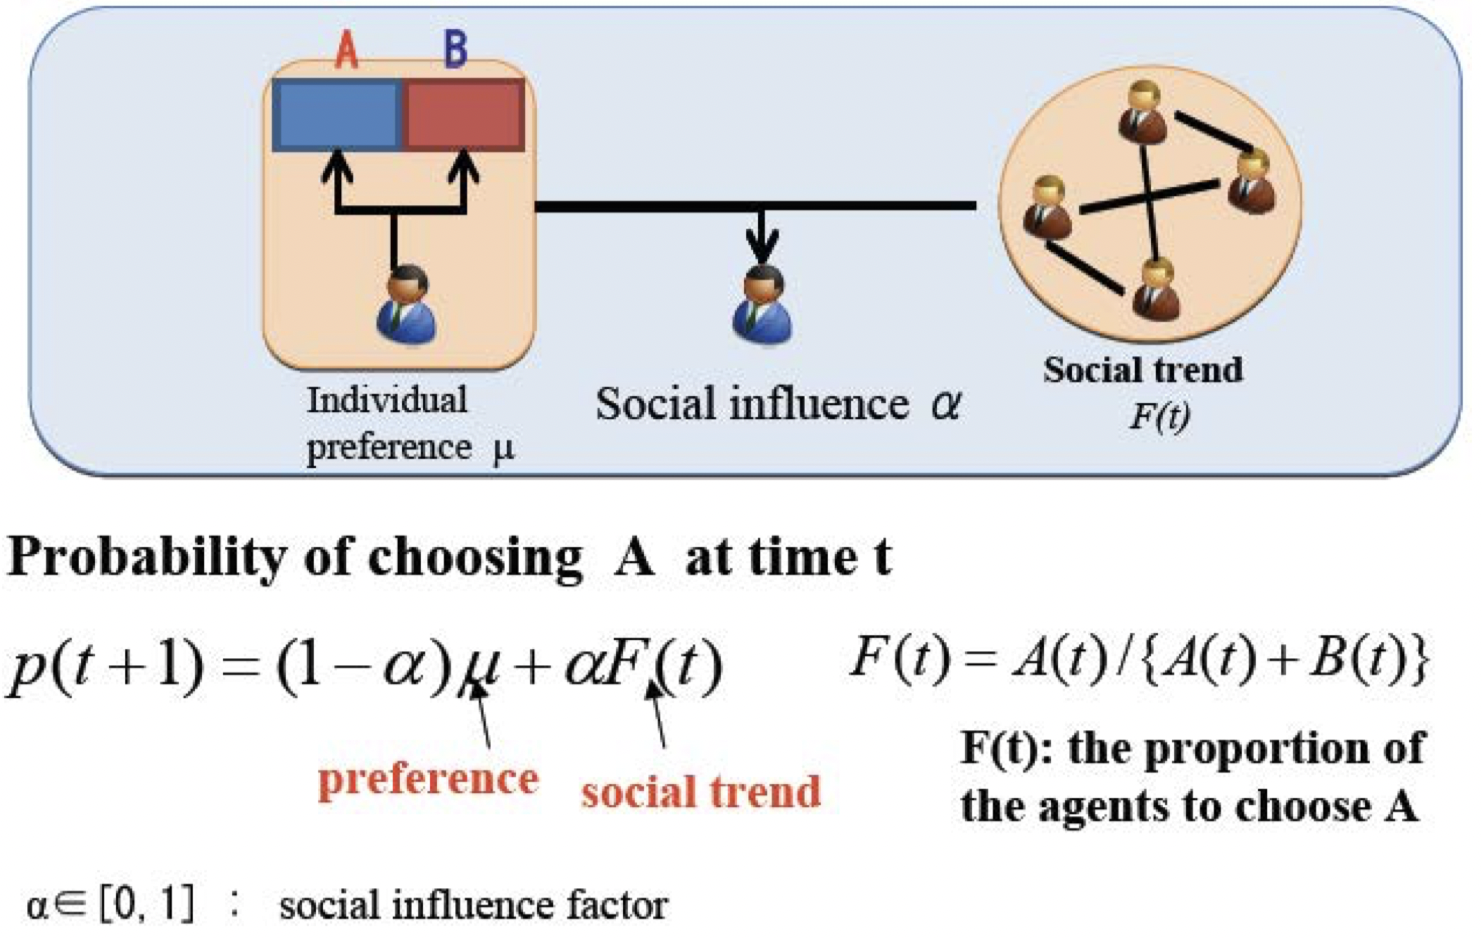
\includegraphics[width=11cm]{../images/EnpRisk_Fig7-1}
    \centering
\end{figure}

More intuitively:

\begin{itemize}
    \item No personal preference and only social interaction: $\mu = 0, \, F(t + 1) = F(t) + \alpha \cdot F(t) \cdot (1 - F(t))$
    \item Only personal preference and no social interaction: $\alpha = 0, \, F(t + 1) = F(t) + \mu \cdot (1 - F(t))$
\end{itemize}

The following figure shows an example with $\mu = 0.5$:

\begin{figure}[H]
    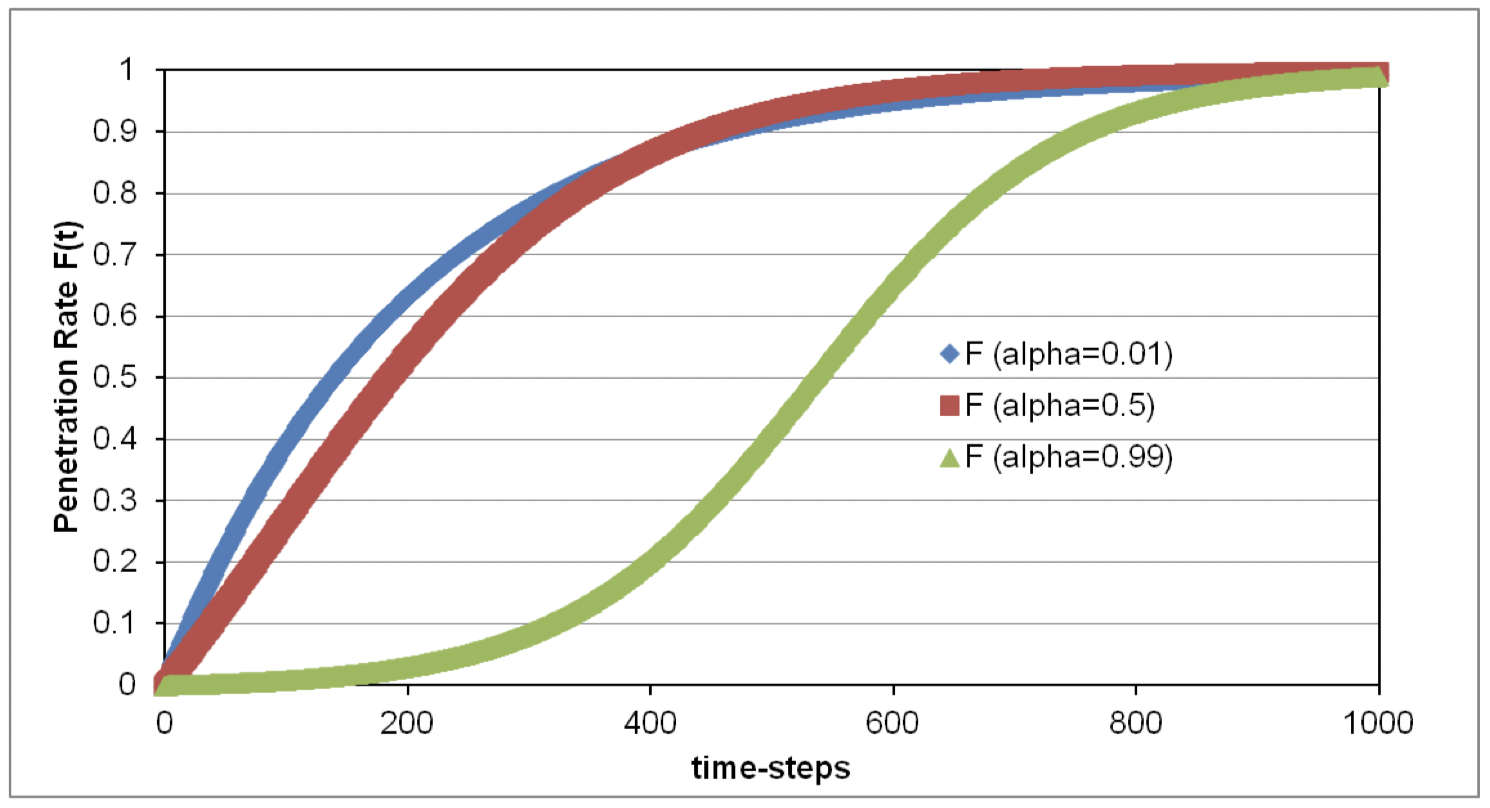
\includegraphics[width=13cm]{../images/EnpRisk_Fig7-2}
    \centering
\end{figure}

\subsection{Case Study: Valuation of Facebook}

The methodology works as follows:

\begin{itemize}
    \item We model the Monthly Active Users: $MAU(t)$
    \item We model the revenues per user: $r(t)$
    \item We define a profit margin: $p$
    \item \textit{Profits at time:} $r(t) \cdot MAU(t) \cdot p$
    \item We define the value of the company as the sum of all the discounted future profits using a discount rate $d$
\end{itemize}

In the end, we have:

\[
    valuation = \sum_{t = 1}^{end} \frac{r(t)MAU(t)p}{(1 + d)^t} = \sum_{t = 1}^{end} \frac{profits(t)}{(1 + d)^t}
\]

In conclusion, we have developed a new methodology to compute the fundamental value of social networking companies based on the dynamics of their users and revenues per user:

\begin{figure}[H]
    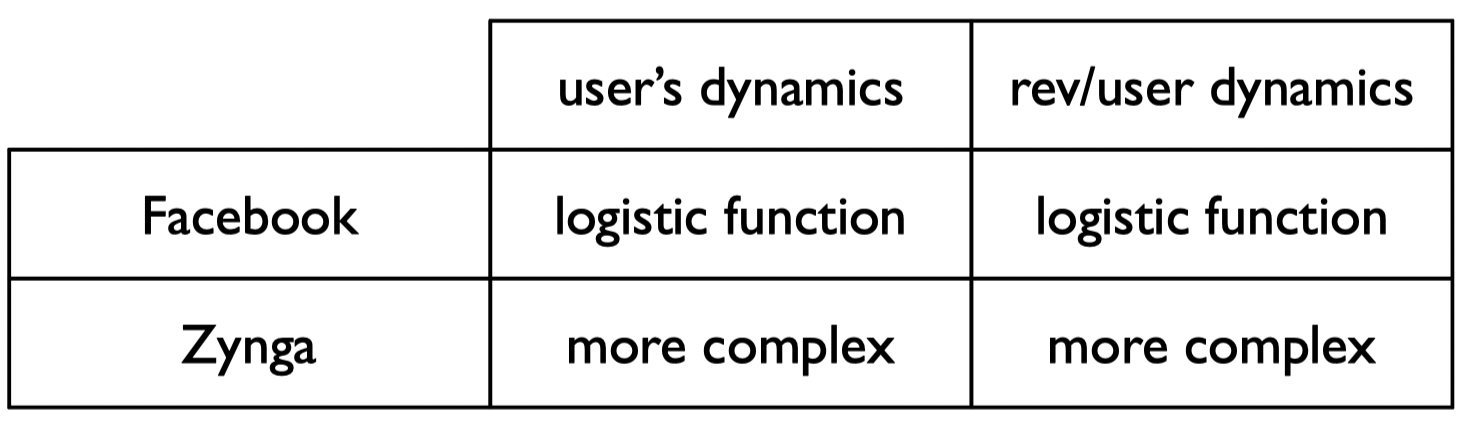
\includegraphics[width=11cm]{../images/EnpRisk_Fig7-3}
    \centering
\end{figure}

Based on that, we can compute the intrinsic value of social networking companies.

The three \textit{important laws of valuation and investment are:}

\begin{itemize}
    \item Prediction is no extrapolation, but understanding the underlying process.
    \item Understand the technicalities of the market and of investment banking.
    \item Always \textbf{RTFM - Read The Fucking Manual!}
\end{itemize}

\end{document}